\chapter{Learning-Based Recognition of Human-Grasped Objects}
\label{chapter:learning}

\textcolor{red}{needs a better chapter introduction} This chapter covers this dissertation's learning part, including data collecting, dataset preprocessing, and the models' structures and optimizations.

\section{Proposal Overview}

\subsection{Problem Description and Formulation \textcolor{red}{(Must be changed)}}

When anticipating the next action of the user, the object that the user is grasping can provide crucial information about the user's intention. Although an object detection algorithm may be helpful they can suffer from occlusion problems. Therefore, the following models attempt to solve this problem by taking an image of the user grasping a certain object and classifying which object is being grasped using the geometry of the hand.

To obtain a model that would be able to achieve the previous objective two experiments were made. In the first experiment, some types of models were tested with a smaller dataset containing only 300 images per object and 3 objects with the aim of knowing if they would be worth using and optimizing in a more complex problem. In the second experiment, a bigger dataset with 3000 images per object and 4 objects was used to train and optimize the models.

\begin{figure}[H]%[!ht]
    \centering
    \begin{tikzpicture}[>=latex']
    \tikzset{block/.style= {draw, rectangle, align=center,minimum width=1.5cm,minimum height=1.5cm},
    rblock/.style={draw, shape=rectangle,rounded corners=1.5em,align=center,minimum width=2cm,minimum height=1cm},
    input/.style={ % requires library shapes.geometric
    draw,
    trapezium,
    trapezium left angle=60,
    trapezium right angle=120,
    minimum width=2cm,
    align=center,
    minimum height=1cm
    },
    }
    
    \node [rblock] (camera) {Camera\\Image};
    \node [block, above =1cm of camera] (hands_keypoints) {Mediapipe\\Hands Model};
    \node [block, below =1cm of camera] (body_keypoints) {Mediapipe\\Pose Model};
    \node [block, right =0.5cm of camera] (right_hand_keypoints_detection) {Right Hand\\Keypoints\\Detection};
    \node [block, right =2cm of right_hand_keypoints_detection] (normalization) {Points\\Normalization};
    \node [block, right =2cm of normalization] (model) {Model\\Prediction};
    \node [rblock, right =0.25cm of model] (output) {Predicted\\Object};
    %\node [below left =0.1cm of normalization] (image1) {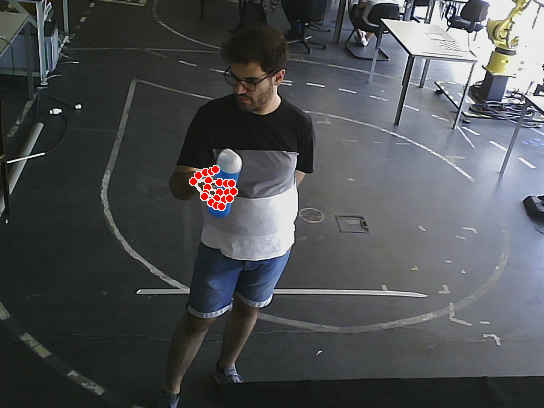
\includegraphics[width=.15\textwidth]{figs/dataset_preprocessing2_1.png}};
    %\node [below left =0.1cm of model] (image2) {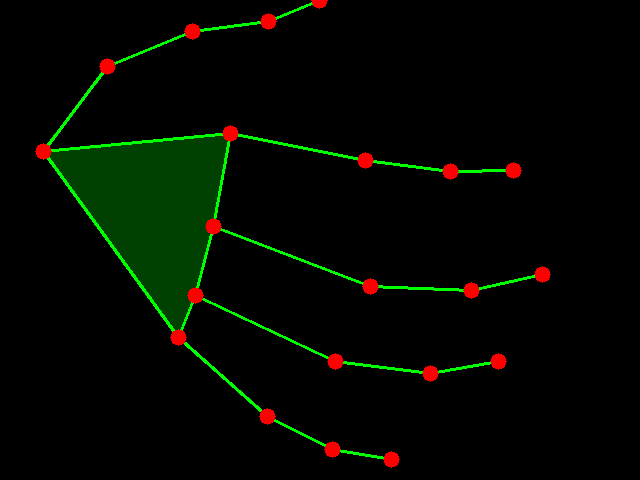
\includegraphics[width=.15\textwidth]{figs/dataset_preprocessing3_1.png}};

    \path[draw,->, text width=2cm, align=center]
                (camera) edge (hands_keypoints)
                (camera) edge (body_keypoints)
                (hands_keypoints) edge node[right, near start] {Hands\\Keypoints} (right_hand_keypoints_detection)
                (body_keypoints) edge node[right, near start] {Pose\\Keypoints} (right_hand_keypoints_detection)
                (right_hand_keypoints_detection) edge node[below] {\adjincludegraphics[width=.9\textwidth, trim={{.25\width} {0.25\height} {.25\width} {0.25\height}}, clip]{figs/dataset_preprocessing2_1.png}} (normalization)
                (normalization) edge node[below] {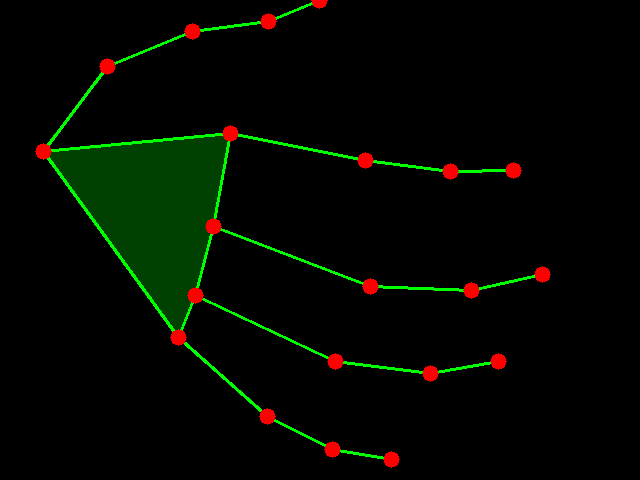
\includegraphics[width=.9\textwidth]{figs/dataset_preprocessing3_1.png}} (model)
                (model) edge (output)
                ;

    %% paths
    \if{0}
    \path[draw,->, text width=3cm, align=center]
                (camera) edge (hands_keypoints)
                (camera) edge[bend right] (body_keypoints)
                (hands_keypoints) edge node[above] {{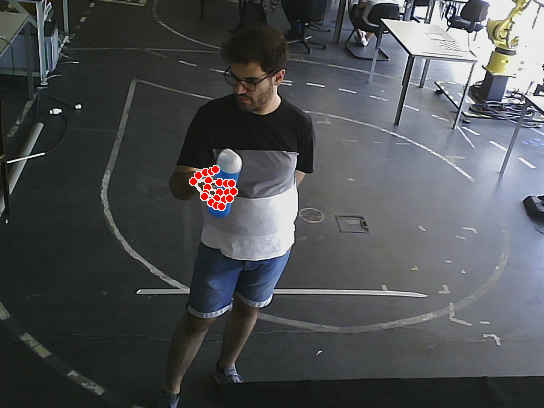
\includegraphics[width=.9\textwidth]{figs/dataset_preprocessing2_1.png}}} (body_keypoints)
                (body_keypoints) edge node[right] {right hand keypoints} (normalization) 
                (normalization) edge node[above] {normalized right hand keypoints} (model)
                (model) edge (output)
                ;
    \fi

    \if{0}
    \node [rblock] (camera) {Camera\\Image};
    \node [block, right =0.5cm of camera] (hands_keypoints) {Mediapipe\\Hands\\Model};
    \node [block, right =0.5cm of hands_keypoints] (body_keypoints) {Mediapipe\\Full Body\\Model};
    \node [block, right =0.5cm of body_keypoints] (normalization) {Points\\Normalization};
    \node [block, right =0.5cm of normalization] (model) {Model\\Prediction};
    \node [rblock, right =0.5cm of model] (output) {Predicted\\Object};

    %% paths
    \path[draw,->, text width=1.7cm, align=center]
                (camera) edge (hands_keypoints)
                (camera) edge[bend right] (body_keypoints)
                (hands_keypoints) edge (body_keypoints)
                (body_keypoints) edge (normalization) 
                (normalization) edge (model)
                (model) edge (output)
                ;
    \fi
    
\end{tikzpicture}
    \caption{Machine Learning Pipeline}
    \label{fig:ml_pipeline}
\end{figure}

\subsection{Evaluation Metrics}

To properly ascertain the performance and generalization capability of deep learning models, metrics must be employed. Accuracy is one of the most widely used metrics in the realm of deep learning, representing the percentage of correct model predictions: \begin{equation}A=\frac{Number\ of\ Correct\ Predictions}{Total\ Number\ of\ Predictions}\label{eq:acc}\end{equation}

Although accuracy clearly assesses the model's performance, it may not be recommended in some situations, like when working with an imbalanced dataset. Therefore other metrics should be used, such as:

\begin{itemize}
    \item True Positive (TP) - instances correctly classified as positive;
    \item True Negative (TN) - instances correctly classified as negative;
    \item False Positive (FP) - instances incorrectly classified as positive;
    \item False Negative (FN) - instances incorrectly classified as negative.
    \item Positive Predictive Value (PPV) or Precision, which is the percentage of instances correctly classified as positive relative to all instances classified as positive: \begin{equation}PPV=\frac{TP}{TP+FP}\label{eq:ppv}\end{equation}
    \item True Positive Rate (TPR) or Recall, which is the percentage of positive instances that are classified as positive: \begin{equation}TPR=\frac{TP}{TP+FN}\label{eq:tpr}\end{equation}
    \item F1-Score, which is the harmonic mean between the precision and the recall: \begin{equation}TPR=2\frac{PPV*TPR}{PPV+TPR}=\frac{2TP}{2TP+FP+FN}\label{eq:f1-score}\end{equation}
\end{itemize}

Precision is a relevant metric to use when the aim is to minimize false positives, while Recall is relevant to minimize false negatives. F1-Score includes the two of them, with both false positives and false negatives having influence over the result.

In a multi-class classification problem, such as the one in this work, these metrics are obtained separately for each class and then averaged across all classes to obtain a final metric. \textcolor{red}{(it might be a good idea to define macro and micro averaging)}

In addition to the previous metrics, a Confusion Matrix can be used to visually represent the model's performance in a tabular way. Each entry $i,j$ contains the number of instances from the class $i$ that are classified as belonging to the class $j$ (e.g., Fig.~\ref{fig:non-norm_conf_matrix}). A confusion matrix can also undergo normalization by dividing each entry by the sum of its row so that each entry provides ratios instead (e.g., Fig.~\ref{fig:norm_conf_matrix}).

\begin{figure}[H]
    \centering
    \begin{subfigure}[b]{0.48\textwidth}
        {\fontsize{10}{12}\selectfont\includesvg[width=\textwidth]{figs/conf_matrix_example2.svg}}
        \caption{Non-normalized Confusion Matrix}
        \label{fig:non-norm_conf_matrix}
    \end{subfigure} \
    \begin{subfigure}[b]{0.48\textwidth}
        {\fontsize{10}{12}\selectfont\includesvg[width=\textwidth]{figs/conf_matrix_example.svg}}
        \caption{Normalized Confusion Matrix}
        \label{fig:norm_conf_matrix}
    \end{subfigure}
    \caption[Confusion Matrix Examples]{Confusion Matrix Examples}
    \label{fig:conf_matrix_examples}
\end{figure}

\section{Data Representation}

\subsection{Dataset Acquisition}

The first step to train a supervised machine learning model is to find a dataset. However, given that this problem is particular, the datasets had to be manually collected. For this purpose, two datasets were collected, consisting of videos where one person would move and rotate a particular object. These videos were recorded using the Orbbec Astra Pro, positioned in front of the user at ten frames per second to avoid consecutive frames with similar hand poses. Fig.~\ref{fig:dataset_examples} shows some examples in the second dataset.

\begin{figure}[H]
    \centerline{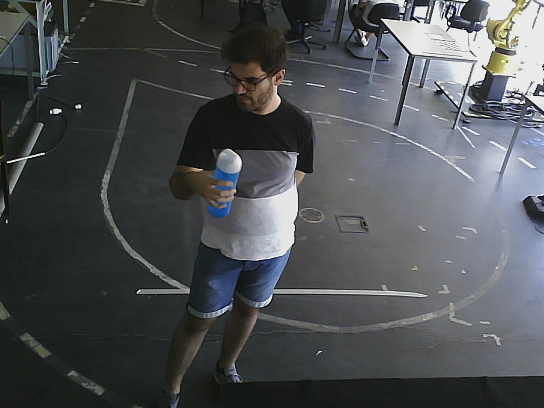
\includegraphics[width=0.49\textwidth]{figs/dataset_preprocessing1_1.png} 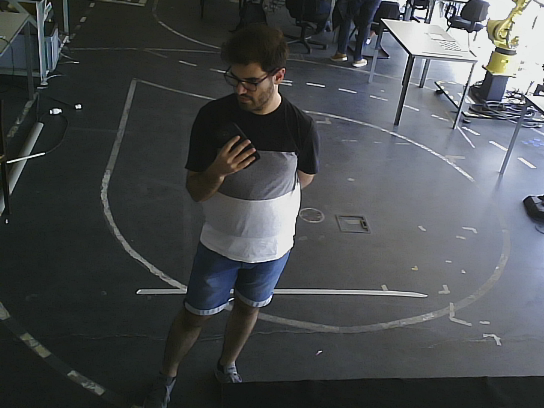
\includegraphics[width=0.49\textwidth]{figs/dataset_preprocessing1_2.png}}
    \caption[Dataset Examples]{Dataset Examples}
    \label{fig:dataset_examples}
\end{figure}

The datasets were captured using the usb\_cam package for ROS, and the videos were saved as bag files. In the first dataset, three different objects were used (see Fig.~\ref{fig:objects_dataset1}), and for each one, one person was recorded for 30 seconds resulting in 300 images per object. In the second dataset, four objects were used (see Fig.~\ref{fig:objects_dataset2}), and three people were recorded in 4 different 25-second videos for each object resulting in 1000 frames for each person and object, making it 3000 frames for each object. Recording more than one video for each combination of person and object allowed each person to grasp the object slightly differently each time in order to obtain a more diverse dataset.

\begin{figure}[H]
    \centering
    \begin{subfigure}[b]{0.49\textwidth}
        \includegraphics[width=\textwidth]{figs/objects_dataset1.jpg}
        \caption{First Dataset Objects}
        \label{fig:objects_dataset1}
    \end{subfigure} \
    \begin{subfigure}[b]{0.49\textwidth}
        \includegraphics[width=\textwidth]{figs/objects_dataset2.jpg}
        \caption{Second Dataset Objects}
        \label{fig:objects_dataset2}
    \end{subfigure}
    \caption[Dataset Objects]{}
    \label{fig:dataset_objects}
\end{figure}

\subsection{Preprocessing}

After having a dataset, the data had to be processed to have a fitting structure to be used in the model training. The images from the videos were processed using the Mediapipe hands model resulting in 21 points for each hand detected, as shown in Fig.~\ref{fig:dataset_examples2}.

\begin{figure}[H]
    \centerline{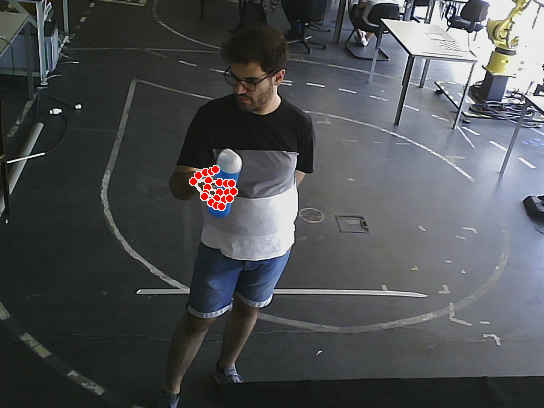
\includegraphics[width=0.49\textwidth]{figs/dataset_preprocessing2_1.png} 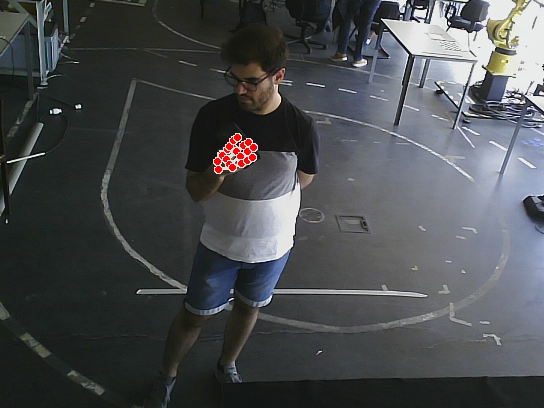
\includegraphics[width=0.49\textwidth]{figs/dataset_preprocessing2_2.png}}
    \caption[Points detected on the Pictures in Fig.~\ref{fig:dataset_examples} by Mediapipe Hands Model]{Points detected on the Pictures in Fig.~\ref{fig:dataset_examples} by Mediapipe Hands Model}
    \label{fig:dataset_examples2}
\end{figure}

The Mediapipe Hands Model can detect a variable number of hands in an image, and it was set up so that it would only detect up to two hands, meaning that its output can consist of no hands detected, of a set of 21 points hand detected, which can be either the left or the right hand, or two sets of 21 points if both hands were detected. To better understand the Mediapipe results in this particular context, six videos with 250 frames each were recorded in different scenarios. Then, for each scenario, the full-body model provided by MediaPipe was used to register whether the model detected the left hand, right hand, both hands, or none, resulting in the metrics in Table \ref{table:mediapipe_metrics}. These results show that there is a significant number of frames where the right hand, which is the one holding the object, is not detected. This means that the results of the Hands Model must be filtered to avoid wrong predictions.

\begin{table}[H]
    \centering
    \caption{Mediapipe Hand Model Output Percentage in Different Scenarios}
    \label{table:mediapipe_metrics}
    \begin{tabular}{|l|l|l|l|l|}
        \hline
        & No Hands & Left Hand & Right Hand & Both Hands \\
        \hline
        Hands Visible & 1.6\% & 2\% & 8.8\% & 87.6\% \\
        \hline
        Hand Holding Bottle & 0.4\% & 44.4\% & 22.8\% & 32.4\% \\
        \hline
        Hand Holding Cube & 1.2\% & 22\% & 36.8\% & 40\% \\
        \hline
        Hand Holding Phone & 1.2\% & 28.4\% & 33.6\% & 36.8\% \\
        \hline
        Hand Holding Screwdriver & 1.2\% & 9.2\% & 44.4\% & 48.4\% \\
        \hline
        Hands Obstructed & 38.8\% & 21.6\% & 26.4\% & 13.2\% \\
        \hline
    \end{tabular}
\end{table}

Given that the scope of this work is restricted to scenarios where the user grasps the objects with his right hand, the instances where the right hand is not detected need to be ignored and, as a result, the images are also processed by the pose model provided by Mediapipe so that it is possible to identify the right hand.

In the preprocessing implementation in ROS, each Mediapipe model has a corresponding ROS node that communicates with the others using actions. This communication method ensures that the models can run in parallel with each other and that the node that makes the requests does not need to wait for the results of the first model to make a request to the second as would be the case if services were used. Although communicating using publish/subscribe nodes would also respect the previous requirements, using actions also has the advantage of guaranteeing that the images analyzed by both models are the same.

The points corresponding to the right hand are then subject to further processing and normalization so that the location of the hand in the image and the distance between the hand and the camera have a lesser impact on the model training. Firstly, the centroid is calculated, and the points are translated to be centered in the (0.5, 0.5, 0.5) point. Then the points are scaled up as much as possible while keeping every coordinate of every point between 0 and 1, as shown in Fig.~\ref{fig:dataset_examples3}. It is important to note that throughout the point processing, the order of the points is never changed, and therefore the models can take advantage of this structure.

\begin{figure}[H]
    \centerline{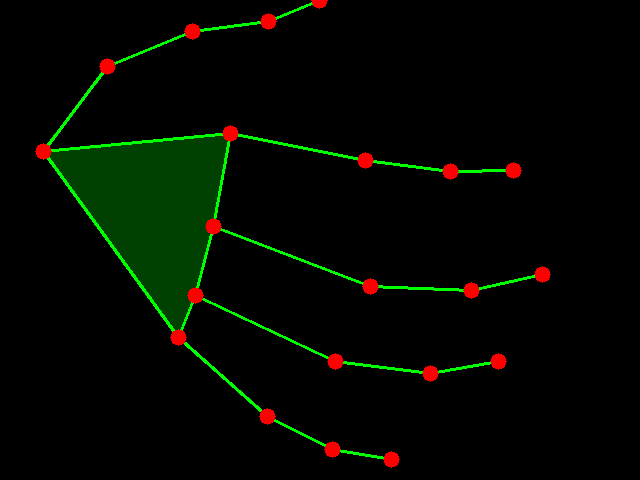
\includegraphics[width=0.49\textwidth]{figs/dataset_preprocessing3_1.png} 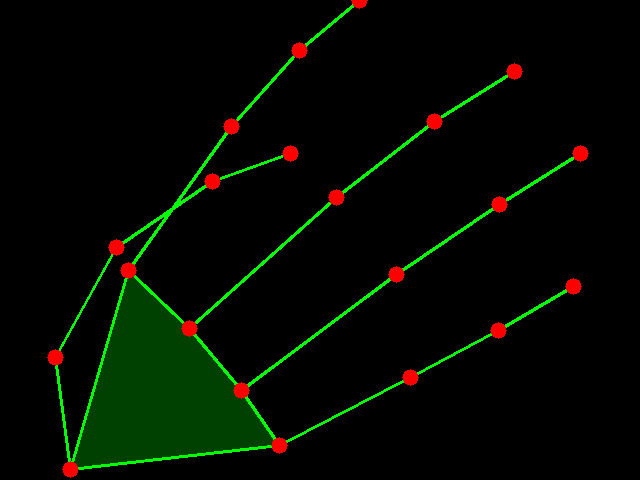
\includegraphics[width=0.49\textwidth]{figs/dataset_preprocessing3_2.png}}
    \caption[Points from the Pictures in Fig.~\ref{fig:dataset_examples2} after Normalization]{Points from the Pictures in Fig.~\ref{fig:dataset_examples2} after Normalization}
    \label{fig:dataset_examples3}
\end{figure}

\subsection{Train-Validation-Test Split}

In order to train the model, the dataset was split into three sets: the train set (60\%), the validation set (20\%), and the test set (20\%). The random variables in the data shuffling and splitting were also fixed so that the test set is always the same, and therefore, its data is never used to train or validate the model, even in different trains. During hyperparameter optimization, the different combinations are tested using 4-fold cross-validation, which means that the model is trained four times, and therefore every sample of data in the initial training and validation set was used both for training and validation. Additionally, early stopping was set up so that the model would stop training after 200 epochs without a better validation loss and restore the best weights.

\section{Convolutional Neural Network Classifier}

Convolutional Neural Networks excel at detecting local relations. Given that each sample provided to the model is made of the 21 points that always follow the same structure representing the right hand, a one-dimensional convolutional neural network was used to take advantage of this characteristic.

\subsection{Model Selection}

For the first dataset, a simple CNN with only one convolutional and one pooling layer was initially tested and manually optimized resulting in the architecture in Fig.~\ref{fig:cnn_architecture_dataset1}.

\begin{figure}[H]
    \centering
    {\fontsize{10}{12}\selectfont\includesvg[width=0.65\textwidth]{figs/cnn_architecture_dataset1.svg}}
    \caption[CNN Model Architecture]{CNN Model Architecture}
    \label{fig:cnn_architecture_dataset1}
\end{figure}

When training a model with this architecture in the second dataset, the results were considerably lower than those achieved with the first dataset. Given that not only was the dataset more extensive, but there was also one more class, it was decided that the model should have a more complex architecture. Therefore, more layers were added resulting in a new architecture.

In addition to the new architecture, three common hyperparameters in CNNs were optimized to obtain even better results. These were the initial learning rate for the model training, the kernel size used by the convolutional layers, and the dropout rate. The number of convolutional layers was also tested alongside them, given that, according to manual testing, it also affected the model results without changing the number of trainable parameters. Table \ref{table:cnn_hyperparameters} shows the values tested for each hyperparameter.

\begin{table}[H]
    \centering
    \caption{Tested Hyperparameter Values}
    \label{table:cnn_hyperparameters}
    \begin{tabular}{|l|l|}
        \hline
        Hyperparameter & Tested Values \\
        \hline
        Learning Rate & 0.01, 0.001, 0.0001 \\
        \hline
        Number of Convolutional Layers & 1, 2, 3 \\
        \hline
        Kernel Size & 2, 3 \\
        \hline
        Dropout Rate & 0.0, 0.1, 0.2, 0.3, 0.4, 0.5 \\
        \hline
    \end{tabular}
\end{table}

In order to choose the best combination of these hyperparameters, all combinations were tested using 4-fold cross-validation, and the average result of each combination was obtained. The combination in Table \ref{table:cnn_best_hyperparameters} resulted in the lowest average loss and an average accuracy of 94.20\%.

\begin{table}[H]
    \centering
    \caption{CNN Best Hyperparameters}
    \label{table:cnn_best_hyperparameters}
    \begin{tabular}{|l|l|}
        \hline
        Hyperparameter & Value \\
        \hline
        Learning Rate & 0.001 \\
        \hline
        Dropout & 0.5 \\
        \hline
        Kernel Size & 3 \\
        \hline
        Number of Convolutional Layers & 2 \\
        \hline
    \end{tabular}
\end{table}

The final model can be seen in Fig.~\ref{fig:cnn_architecture}, and it is made of 2 convolutional layers followed by three dense layers, with the third being the output layer. Between the convolutional and the dense layers and between both dense layers, there is also a dropout layer to help with overfitting.

\begin{figure}[H]
    \centering
    {\fontsize{10}{12}\selectfont\includesvg[width=0.85\textwidth]{figs/cnn_architecture.svg}}
    \caption[CNN Model Architecture]{CNN Model Architecture}
    \label{fig:cnn_architecture}
\end{figure}

\subsection{Performance Evaluation}

\subsubsection{First Dataset}

After the initial architecture was tested and manually optimized with the first dataset, it resulted in the learning curves shown in Fig.~\ref{fig:cnn_dataset1_loss} and Fig.~\ref{fig:cnn_dataset1_acc}. According to the figures, the best validation loss occurred close to the 1800th epoch, with the training stopping 200 epochs later.

\begin{figure}[H]
    \centering
    {\fontsize{10}{12}\selectfont\includesvg[width=\textwidth]{figs/cnn_dataset1_loss_comparison.svg}}
    \caption[CNN training and validation loss evolution during training]{CNN training and validation loss evolution during training}
    \label{fig:cnn_dataset1_loss}
\end{figure}

\begin{figure}[H]
    \centering
    {\fontsize{10}{12}\selectfont\includesvg[width=\textwidth]{figs/cnn_dataset1_acc_comparison.svg}}
    \caption[CNN training and validation accuracy evolution during training]{CNN training and validation accuracy evolution during training}
    \label{fig:cnn_dataset1_acc}
\end{figure}

After the model finished training, the metrics in Table \ref{table:cnn_dataset1_results} were obtained. Given that the test accuracy was over 95\%, we can conclude that the model generalized its knowledge from the training data. Additionally, the confusion matrix in Fig.~\ref{fig:cnn_dataset1_conf_matrix} shows that the model managed to predict more accurately the bottle and the cube, whose shapes are more distinct. Even with a relatively small dataset, this CNN showed positive results, so it was decided that this model should be tested in the second dataset.

\begin{table}[H]
    \centering
    \caption{Metrics obtained with the First Dataset (CNN)}
    \label{table:cnn_dataset1_results}
    \begin{tabular}{|l|l|l|l|l|}
        \hline
        Metric & Accuracy & Precision & Recall & F1-Score \\
        \hline
        Value & 0.9551 & 0.9583 & 0.9551 & 0.9549 \\
        \hline
    \end{tabular}
\end{table}

\begin{figure}[H]
    \centering
    {\fontsize{10}{12}\selectfont\includesvg[width=0.55\textwidth]{figs/cnn_dataset1_conf_matrix.svg}}
    \caption[Confusion Matrix obtained with the First Dataset (CNN)]{Confusion Matrix obtained with the First Dataset (CNN)}
    \label{fig:cnn_dataset1_conf_matrix}
\end{figure}

\subsubsection{Second Dataset}

The final CNN architecture was trained in the second dataset resulting in the training curves in Fig.~\ref{fig:cnn_loss} and Fig.~\ref{fig:cnn_acc}. According to the figures, the best validation loss occurred around the 275th epoch, with the training stopping 200 epochs later.

\begin{figure}[H]
    \centering
    {\fontsize{10}{12}\selectfont\includesvg[width=0.98\textwidth]{figs/cnn_loss_comparison.svg}}
    \caption[CNN training and validation loss evolution during training]{CNN training and validation loss evolution during training}
    \label{fig:cnn_loss}
\end{figure}

\begin{figure}[H]
    \centering
    {\fontsize{10}{12}\selectfont\includesvg[width=0.98\textwidth]{figs/cnn_acc_comparison.svg}}
    \caption[CNN training and validation accuracy evolution during training]{CNN training and validation accuracy evolution during training}
    \label{fig:cnn_acc}
\end{figure}

After the model finished training, the metrics in Table \ref{table:cnn_dataset2_results} were obtained. Given that the test accuracy was over 92\%, we can conclude that the model managed to generalize its knowledge from the training data to classify data it has never seen before. Additionally, the confusion matrix in Fig.~\ref{fig:cnn_dataset2_confusion_matrix} shows that the screwdriver was the object the model managed to predict more accurately. This can be because the hand geometry that allows a person to intuitively grasp a screwdriver is more restricted.

\begin{table}[H]
    \centering
    \caption{Metrics obtained with the Second Dataset (CNN)}
    \label{table:cnn_dataset2_results}
    \begin{tabular}{|l|l|l|l|l|}
        \hline
        Metric & Accuracy & Precision & Recall & F1-Score \\
        \hline
        Value & 0.9236 & 0.9243 & 0.9236 & 0.9237 \\
        \hline
    \end{tabular}
\end{table}

\begin{figure}[H]
    \centering
    {\fontsize{10}{12}\selectfont\includesvg[width=0.75\textwidth]{figs/cnn_conf_matrix.svg}}
    \caption[Confusion Matrix obtained with the Second Dataset (CNN)]{Confusion Matrix obtained with the Second Dataset (CNN)}
    \label{fig:cnn_dataset2_confusion_matrix}
\end{figure}

\section{Transformer Neural Network Classifier}

As said in Subsection \ref{subsection:transformer_neural_networks}, Transformer Neural Networks shine at capturing long-range dependencies and relationships. Therefore, because the points obtained from Mediapipe have a specific order, we can use this ability to process structured data and effectively capture dependencies and patterns.

\subsection{Model Selection}

For the first dataset, a Transformer architecture adapted from an example in the Keras documentation\footnote{Transformer Keras Example: \url{https://keras.io/examples/timeseries/timeseries_transformer_classification}} was tested and manually optimized. The resulting architecture can be seen in Fig.~\ref{fig:transformer_architecture_dataset1} and it is made of four Transformer Encoder Blocks comprised of the layers shown in Fig.~\ref{fig:transformer_encoder_architecture} followed by a Global Average Pooling, a Dense and a Dropout Layer, and a final Dense output layer.

\begin{figure}[H]
    \centering
    {\fontsize{10}{12}\selectfont\includesvg[width=0.8\textwidth]{figs/transformer_encoder.svg}}
    \caption[Transformer Encoder Block]{Transformer Encoder Block}
    \label{fig:transformer_encoder_architecture}
\end{figure}

\begin{figure}[H]
    \centering
    {\fontsize{10}{12}\selectfont\includesvg[width=0.75\textwidth]{figs/transformer_architecture_dataset1.svg}}
    \caption[Transformer Architecture]{Transformer Architecture}
    \label{fig:transformer_architecture_dataset1}
\end{figure}

However, that architecture achieved results significantly lower in the second dataset. After some manual testing, an initial layer was replaced to achieve better results, and the number of trainable parameters was reduced when possible to allow for faster model training.

In addition to the changes in the architecture, three hyperparameters were optimized to improve the performance of the model. These were the initial learning rate for the model training, the dropout rate inside each transformer block, and the dropout rate of the multilayer perception at the end of the model. Table \ref{table:transformer_hyperparameters} shows the values tested for each hyperparameter.

\begin{table}[H]
    \centering
    \caption{Tested Hyperparameter Values}
    \label{table:transformer_hyperparameters}
    \begin{tabular}{|l|l|}
        \hline
        Hyperparameter & Tested Values \\
        \hline
        Learning Rate & 0.01, 0.001, 0.0001 \\
        \hline
        Dropout Rate & 0.0, 0.1, 0.2, 0.3, 0.4, 0.5 \\
        \hline
        MLP Dropout Rate & 0.0, 0.1, 0.2, 0.3, 0.4, 0.5 \\
        \hline
    \end{tabular}
\end{table}

In order to choose the best combination of these hyperparameters, all combinations were
tested using 4-fold cross-validation, and the combination with the smallest average validation loss was chosen. This combination can be seen in Table \ref{table:transformer_best_hyperparameters}
having an average accuracy of 92.24\%.

\begin{table}[H]
    \centering
    \caption{Transformer Best Hyperparameters}
    \label{table:transformer_best_hyperparameters}
    \begin{tabular}{|l|l|}
        \hline
        Hyperparameter & Value \\
        \hline
        Learning Rate & 0.0001 \\
        \hline
        Dropout Rate & 0.5 \\
        \hline
        MLP Dropout Rate & 0.1 \\
        \hline
    \end{tabular}
\end{table}

The final model can be seen in Fig.~\ref{fig:transformer_architecture}, and it is made of two Transformer Encoder Blocks (see Fig.~\ref{fig:transformer_encoder_architecture}) followed by two sets of a Dense and a Dropout Layer and a final Dense output layer.

\begin{figure}[H]
    \centering
    {\fontsize{10}{12}\selectfont\includesvg[width=0.8\textwidth]{figs/transformer_architecture.svg}}
    \caption[Tranformer Model Architecture]{Tranformer Model Architecture}
    \label{fig:transformer_architecture}
\end{figure}

\subsection{Performance Evaluation}

\subsubsection{First Dataset}

After the initial architecture was tested and manually optimized with the first dataset, it resulted in the learning curves shown in Fig.~\ref{fig:transformer_dataset1_loss} and Fig.~\ref{fig:transformer_dataset1_acc}. According to the figures, the best validation loss occurred close to the 300th epoch, with the training stopping 200 epochs later.

\begin{figure}[H]
    \centering
    {\fontsize{10}{12}\selectfont\includesvg[width=0.98\textwidth]{figs/transformer_dataset1_loss_comparison.svg}}
    \caption[Transformer training and validation loss evolution during training]{Transformer training and validation loss evolution during training}
    \label{fig:transformer_dataset1_loss}
\end{figure}

\begin{figure}[H]
    \centering
    {\fontsize{10}{12}\selectfont\includesvg[width=0.98\textwidth]{figs/transformer_dataset1_acc_comparison.svg}}
    \caption[Transformer training and validation accuracy evolution during training]{Transformer training and validation accuracy evolution during training}
    \label{fig:transformer_dataset1_acc}
\end{figure}

After the model finished training, the metrics in Table \ref{table:transformer_dataset1_results} were obtained. Given that the test accuracy was around 90\%, we can conclude that the model generalized its knowledge from the training data. However, the confusion matrix in Fig.~\ref{fig:transformer_dataset1_confusion_matrix} shows that the model managed to predict the bottle and the cube significantly more accurately, whose shapes are more distinct, in comparison with the long block that was mistaken several times for the cube. Even with a relatively small dataset, this Transformer showed positive results even if it showed greater difficulty in distinguishing between two similar objects, so it was decided that this model should be tested in the second dataset.

\begin{table}[H]
    \centering
    \caption{Metrics obtained with the First Dataset (Transformer)}
    \label{table:transformer_dataset1_results}
    \begin{tabular}{|l|l|l|l|l|}
        \hline
        Metric & Accuracy & Precision & Recall & F1-Score \\
        \hline
        Value & 0.8989 & 0.9163 & 0.8989 & 0.9001 \\
        \hline
    \end{tabular}
\end{table}

\begin{figure}[H]
    \centering
    {\fontsize{10}{12}\selectfont\includesvg[width=0.55\textwidth]{figs/transformer_dataset1_conf_matrix.svg}}
    \caption[Confusion Matrix obtained with the First Dataset (Transformer)]{Confusion Matrix obtained with the First Dataset (Transformer)}
    \label{fig:transformer_dataset1_confusion_matrix}
\end{figure}

\subsubsection{Second Dataset}

The final architecture was trained in the second dataset resulting in the training curves in Fig.~\ref{fig:transformer_loss} and Fig.~\ref{fig:transformer_acc}. According to the figures, the best validation loss occurred around the 2700th epoch, with the training stopping 200 epochs later.

\begin{figure}[H]
    \centering
    {\fontsize{10}{12}\selectfont\includesvg[width=0.98\textwidth]{figs/transformer_loss_comparison.svg}}
    \caption[Transformer training and validation loss evolution during training]{Transformer training and validation loss evolution during training}
    \label{fig:transformer_loss}
\end{figure}

\begin{figure}[H]
    \centering
    {\fontsize{10}{12}\selectfont\includesvg[width=0.98\textwidth]{figs/transformer_acc_comparison.svg}}
    \caption[Transformer training and validation accuracy evolution during training]{Transformer training and validation accuracy evolution during training}
    \label{fig:transformer_acc}
\end{figure}

After the model finished training, the metrics in Table \ref{table:transformer_dataset2_results} were obtained. Given that the test accuracy was over 92\%, we can conclude that the model managed to generalize its knowledge from the training data to classify data it has never seen before. Additionally, the confusion matrix in Fig.~\ref{fig:transformer_dataset2_confusion_matrix} shows that the screwdriver was the object the model managed to predict more accurately. This can be because the hand geometry that allows a person to intuitively grasp a screwdriver is more restricted.

\begin{table}[H]
    \centering
    \caption{Metrics obtained with the Second Dataset (Transformer)}
    \label{table:transformer_dataset2_results}
    \begin{tabular}{|l|l|l|l|l|}
        \hline
        Metric & Accuracy & Precision & Recall & F1-Score \\
        \hline
        Value & 0.9244 & 0.9244 & 0.9244 & 0.9243 \\
        \hline
    \end{tabular}
\end{table}

\begin{figure}[H]
    \centering
    {\fontsize{10}{12}\selectfont\includesvg[width=0.75\textwidth]{figs/transformer_conf_matrix.svg}}
    \caption[Confusion Matrix obtained with the Second Dataset (Transformer)]{Confusion Matrix obtained with the Second\\Dataset (Transformer)}
    \label{fig:transformer_dataset2_confusion_matrix}
\end{figure}

\section{Comparative Analysis of Deep Models}

In order to compare the models, they were evaluated in three different cases using different data for model training and testing.

\subsubsection{First Case}

The first case corresponds to the method the models were tested in the previous sections. This means that all data was randomly split into the training and test sets resulting in the metrics shown in Table \ref{table:results_first_case}. These results show both models having similar performances of over 92\%.

\begin{table}[H]
    \centering
    \caption{First Case Results}
    \label{table:results_first_case}
    \begin{tabular}{|l|l|l|l|l|}
        \hline
        Model & Accuracy & Precision & Recall & F1-Score \\
        \hline
        CNN & 0.9236 & 0.9243 & 0.9236 & 0.9237 \\
        \hline
        Transformer & \textbf{0.9244} & \textbf{0.9244} & \textbf{0.9244} & \textbf{0.9243} \\
        \hline
    \end{tabular}
\end{table}

\subsubsection{Second Case}

In the second case, the model was trained once for each user present in the dataset and, on each training, only the data collected with one user was used for both training and testing, resulting in the metrics in the tables \ref{table:results_second_case}. These results show that when testing with only one user, the results with the CNN are similar, but those with the Transformer are slightly lower. One justification could be that even with less variety in the data, the fact that there are fewer samples of data might counterbalance that. Given that the Transformers tend to need more training data, this also justifies the difference in the accuracy.

\begin{table}[H]
    \centering
    \caption{Results in the Second Case}
    \label{table:results_second_case}
    \begin{tabular}{|l|l|l|l|l|l|}
        \hline
        Metric & Model & User1 & User2 & User3 & Average \\
        \hline \hline
        \multirow{2}{*}{Accuracy} & CNN & \textbf{0.9577} & \textbf{0.9068} & \textbf{0.9026} & \textbf{0.9224} \\
        \cline{2-6}
        & Transformer & 0.9400 & 0.8892 &  0.8660 & 0.8984 \\
        \hline \hline
        \multirow{2}{*}{Precision} & CNN & \textbf{0.9580} & \textbf{0.9069} & \textbf{0.9029} & \textbf{0.9226} \\
        \cline{2-6}
        & Transformer & 0.9404 & 0.8894 & 0.8675 & 0.8991 \\
        \hline \hline
        \multirow{2}{*}{Recall} & CNN & \textbf{0.9577} & \textbf{0.9068} & \textbf{0.9026} & \textbf{0.9224} \\
        \cline{2-6}
        & Transformer & 0.9400 & 0.8892 & 0.8660 & 0.8984 \\
        \hline \hline
        \multirow{2}{*}{F1-Score} & CNN & \textbf{0.9577} & \textbf{0.9068} & \textbf{0.9025} & \textbf{0.9223} \\
        \cline{2-6}
        & Transformer & 0.9399 & 0.8892 & 0.8663 & 0.8985 \\
        \hline
    \end{tabular}
\end{table}

\subsubsection{Third Case}

In the third case, the model was also trained once for each user in the dataset. However, this time, the model was trained with the data collected from two users, with the data from the third being used for testing resulting in the metrics in the tables \ref{table:results_third_case}. These results show that testing with a user whose data was not used to train a model produces significantly lower results. This can be justified due to different people grasping objects in different ways. Additionally, since the dataset is made of data derived from only three people, removing one from the training data significantly reduces the variety of the training data.

\begin{table}[H]
    \centering
    \caption{Results in the Third Case}
    \label{table:results_third_case}
    \begin{tabular}{|l|l|l|l|l|l|}
        \hline
        Metric & Model & User1 & User2 & User3 & Average \\
        \hline \hline
        \multirow{2}{*}{Accuracy} & CNN & \textbf{0.7879} & \textbf{0.5751} & \textbf{0.5444} & \textbf{0.6358} \\
        \cline{2-6}
        & Transformer & 0.7655 & 0.5686 & 0.5309 & 0.6217 \\
        \hline \hline
        \multirow{2}{*}{Precision} & CNN & \textbf{0.8036} & \textbf{0.5834} & \textbf{0.5567} & \textbf{0.6479} \\
        \cline{2-6}
        & Transformer & 0.7808 & 0.5776 & 0.5553 & 0.6371 \\
        \hline \hline
        \multirow{2}{*}{Recall} & CNN & \textbf{0.7879} & \textbf{0.5751} & \textbf{0.5444} & \textbf{0.6358} \\
        \cline{2-6}
        & Transformer & 0.7655 & 0.5686 & 0.5309 & 0.6217 \\
        \hline \hline
        \multirow{2}{*}{F1-Score} & CNN & \textbf{0.7915} & \textbf{0.5710} & \textbf{0.5417} & \textbf{0.6347} \\
        \cline{2-6}
        & Transformer & 0.7681 & 0.5648 & 0.5312 & 0.6214 \\
        \hline
    \end{tabular}
\end{table}

\subsubsection{Summary}

From the three cases evaluated, the CNN performed better in situations requiring more generalization capability and with less data, such as the second and third cases. However, in the first case, the Transformer obtained similar metrics, while in the other cases, the metrics were lower by a relatively small difference. From the confusion matrixes in Fig.~\ref{fig:cnn_dataset2_confusion_matrix} and Fig.~\ref{fig:transformer_dataset2_confusion_matrix} we can also see that the Transformer has a more consistent performance across all classes in comparison with the CNN which shows higher differences between per-class accuracies. Given that a key difference in the second and third cases is the amount of data, this may mean that, with a bigger dataset, the performance of the Transformer might surpass the CNN.

\section{Human Intention Prediction in Shared Tasks}

\textcolor{red}{(What should be the content of this section? Is it the integration in the system described in the last chapter)}

\section{Final Remarks}